\documentclass[10pt,a4paper]{report}
\usepackage{pdflscape} %Landscape format
\usepackage[T1]{fontenc}
\usepackage{graphicx}
\usepackage{subcaption}
\usepackage[ddmmyyyy]{datetime}
\usepackage{adjustbox}
\graphicspath{ {./images/} }
%\usepackage{natbib}
\renewcommand{\bibname}{Kaynakça}



\title{Kalabalık Sayımı/Tespiti }
\date{\today}
\author{Baki Dinç}
\renewcommand\thesection{\arabic{section}}

\begin{document}
	\textbf{KÜTAHYA SAĞLIK BİLİMLERİ ÜNİVERSİTESİ}\centering
	\begin{figure}[!h]
		\centering
		
\includegraphics{ksbu}
		\maketitle
	\end{figure}
	
	
	\newpage
	
	\raggedright\section*{1.Giriş}
	\raggedright
Teknolojinin gelişimi, özellikle yapay zeka ve derin öğrenme alanındaki ilerlemeler, günlük yaşantımızdaki birçok alanda çeşitli çözümler sunmaktadır. Bu kapsamda, "Kalabalık Sayımı/Tespiti" adlı Projem, bir alışveriş merkezindeki kalabalığın veya merkezi bir caddede bulunan insanların (kalabalığın) sayılması üzerine odaklanmaktadır.\newline



Bu proje ortak bir amacı, kalabalık alanlarda bulunan insan sayısını doğru ve etkili bir şekilde tespit ederek, çeşitli alanlarda güvenlik, operasyonel verimlilik, pazarlama stratejileri, salgın kontrolü ve müşteri deneyimi gibi çeşitli konularda kullanılabilecek veriler üretmektir.\newline



Proje, bir gözetleme kamerası tarafından kaydedilen görüntüler üzerinde derin öğrenme tekniklerini kullanarak kalabalığı saymayı amaçlamaktadır.
Bu projenin temel amaçlardan biri kalabalık ortamlarda kişi sayısını tahmin edip kalabalık ortamlarda alınabilecek tedbirlere ve kalabalığı yönlendirmeye veya korumaya yönelik tedbirler almaktır.\newline



	\raggedright\section*{2.Literatür Araştırması}
	
	Evrişimsel Sinir Ağları hakkında bilgi edinmek amacıyla  MIT 6.S191: Introduction to Deep Learning Youtube Playlistinden  Alexander Amini'nin anlatımıyla  Evrişimsel Sinir Ağları videosu\cite{amini2022cnnvideo}. izlenilmiştir.\newline
	
	CNN'ler hakkında bilgi sahibi olmak amacıyla IBM Technology'nin yayınladığı  What are Convolutional Neural Networks (CNNs) ?\cite{cnnvideo}  youtube videosundan yararlanılmıştır.\newline
	
	
	Object Detection 101 Course - Including 4xProjects | Computer Vision başlıklı \cite{Computer_Vision} Youtube video içeriği konu ile alakalı proje kısmında incelenilmelerde bulunulmuştur  . Bu video,  nesne tespiti (Object Detection) konusunu ele alıyor.
	
	Bu çalışmada, modelimizin performansını değerlendirmek amacıyla iki farklı veri seti
	 \cite{CrowdCounting_dataset1}.\cite{CrowdCounting_dataset2}.   kullanılacaktır   Her bir veri seti, eğitim, test ve doğrulama aşamalarını içeren ayrı ayrı bölümlere tabi tutulmuştur.\newline
	\\
	Kalabalık sayma alanındaki  çalışmalardan biri de Shoval T. tarafından yapılan ve Kaggle platformunda paylaşılan Keras ön eğitimli ResNet50 CNN uygulamasıdır. Bu çalışma, CNN'lerin kalabalık saymada kullanımına dair somut bir örnek sunar\cite{shovalt2018crowdcounting}.. \newline
	
	Shoval T.'nin yaklaşımı, derin öğrenme alanında yaygın olarak kullanılan Keras kütüphanesi ve ImageNet üzerinde önceden eğitilmiş güçlü bir CNN mimarisi olan ResNet50 üzerine inşa edilmiştir.\newline
	
	\clearpage
	Proje kapsamında incelenen bir başka veri modeli, Rahul Mishra (2019) tarafından sunulan CNN ile kalabalık sayma- sosyal mesafe \cite{RahulMishra} projesi yanı sıra Rahul Mishra (2019) tarafından sunulan sosyal mesafe projesinde kullanılan CNN modeli incelenmiştir.\newline
	
		
	Proje kapsamında incelenen bir başka veri modeli ,Veri Modeli, Chao Zhuang (2024) tarafından sunulan People Statistics: Traffic Control in a Mall \cite{ChaoZhuang}  tarafından sunulan, kullanılan Algoritma  modeli incelenmiştir.	\newline
	


	Rapor içerisinde yer alan bazı metinsel ifadelerde dil modeli olarak OpenAI'nin GPT-3.5 tabanlı bir modelinden faydalanılmıştır\cite{chatgpt_dilmodeli} ve  Google AI tarafından geliştirilen Gemini dil modeli kullanılmıştır\cite{gemini}.	\newline
	

   Kullanılan \cite{CrowdCounting_dataset1} veri setinde toplanılan bilgiler ve kaynaklar :\cite{change2013semi}\cite{chen2013cumulative}\cite{loy2013crowd}\cite{chen2012feature}\newline
	
   Proje Veri Modelleri ve dataset içeren paperswithcode.com sitesinden  ShanghaiTech\cite{ShanghaiTech} incelenmiştir.


\newpage
\raggedright\section*{3. Metodoloji}

		\begin{enumerate}
			
		\item[\textbf{3.1}] \textbf{Veri Setinin Yüklenmesi} \\
				Etiketler .csv dosyasından yüklenecektir.
				Görüntüler images.npy dosyasından yüklenir ve numpy dizisine dönüştürülür.
		
		 	\item[\textbf{3.2}] \textbf{Transfer Öğrenme} \\
		Kod, önceden eğitilmiş ResNet50 modelini veya başka bir modeli kullanarak transfer öğrenme yöntemini benimseyecektir. Bu, ImageNet veri kümesinde eğitilmiş bir modelin, başka bir görevde (burada kalabalık sayma) kullanılması anlamına gelir.
		
		 	\item[\textbf{3.3}] \textbf{Veri Ön İşleme} \\
		veri ön işleme gerçekleştirilir. ResNet50 veya başka bir modeli için önceden tanımlanmış olan giriş görüntülerini modele uygun formata getirilir.
		
	\item[\textbf{3.4}] \textbf{Model Modifikasyonu} \\
		Önceden eğitilmiş ResNet50 modeli, başka bir görev için uyarlanmak üzere değiştirilir. Yeni eklenen katmanlar, modelin kalabalık sayma problemine uyarlanmasını sağlar.
		
	\item[\textbf{3.5}] \textbf{Regresyon} \\
		kalabalık sayma probleminde regresyon kullanılabilir. Giriş olarak bir görüntü alınabilir ve çıktı olarak bu görüntüdeki insan sayısı (sürekli bir sayı) tahmin edilebilir. Bu nedenle, regresyon, bağımlı değişkenin sürekli bir değer olduğu problemleri çözmek için uygundur.
		
		
	\item[\textbf{3.7}] \textbf{Modelin Oluşturulması ve Eğitimi} \\
		Basit bir evrişimli sinir ağı (CNN) modeli oluşturulur.        
		
	\item[\textbf{3.8}] \textbf{Modelin İyileştirilmesi} \\
		İlk eğitim sonrasında, modelin performansını iyileştirmek için öğrenme hızı ve epoch sayısı gibi hiperparametreler ayarlanabilir.
		
	\item[\textbf{3.9}] \textbf{Sonuçların Görselleştirilmesi} \\
		Eğitim sürecinin sonuçları, epoch'a bağlı olarak öğrenme hızının değişimini gösteren bir grafik ile görselleştirilir.
		\item[\textbf{3.10}] \textbf{Kullanılan Teknolojiler-Kütüphaneler } \\	
		Keras\\
		tensorflow\\
		sklearn	\\
		numpy\\
		pandas \\
		seaborn \\
		scipy \\
		matplotlib\\\
		\end{enumerate}
		
		\newpage
		
		
	\begin{figure}[!h]
		\subcaptionsetup{labelformat=empty}
		\begin{itemize}
			\raggedright \item[{}] \textbf{Örnek veriler:}  
		\end{itemize}
		\begin{subfigure}{\textwidth}
			\raggedright
			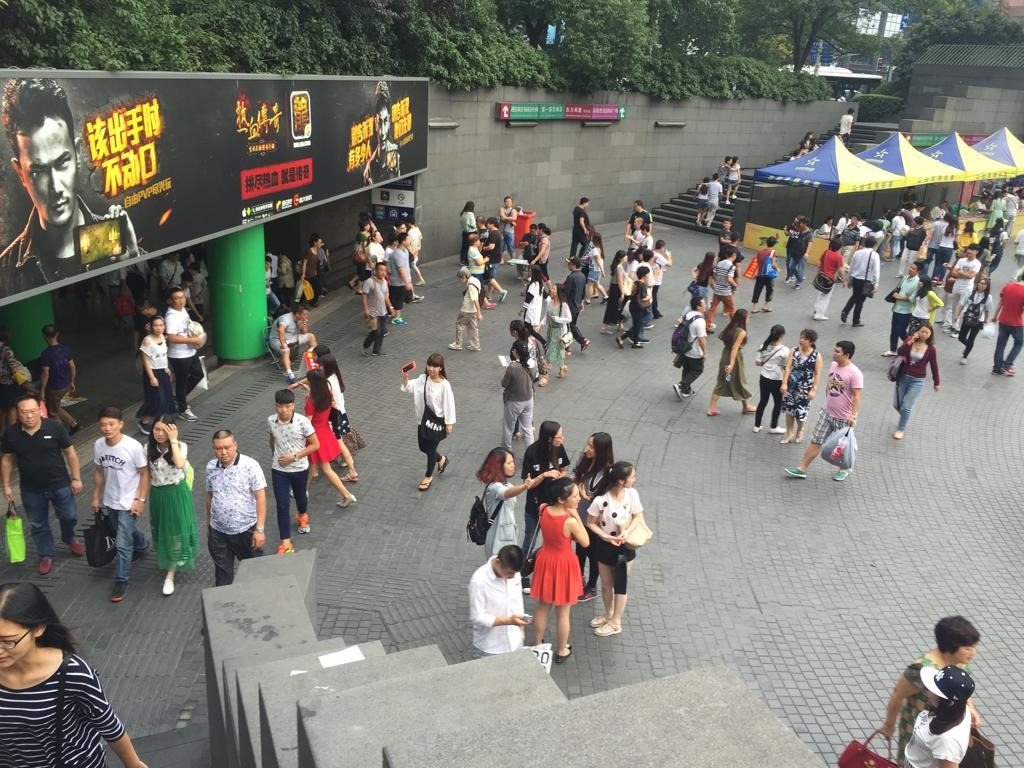
\includegraphics[width=\textwidth]{ornek1.jpg}
			\caption{Örnek 1}
			\label{Ornek1}
		\end{subfigure}
		\begin{subfigure}{\textwidth}
			\raggedright
			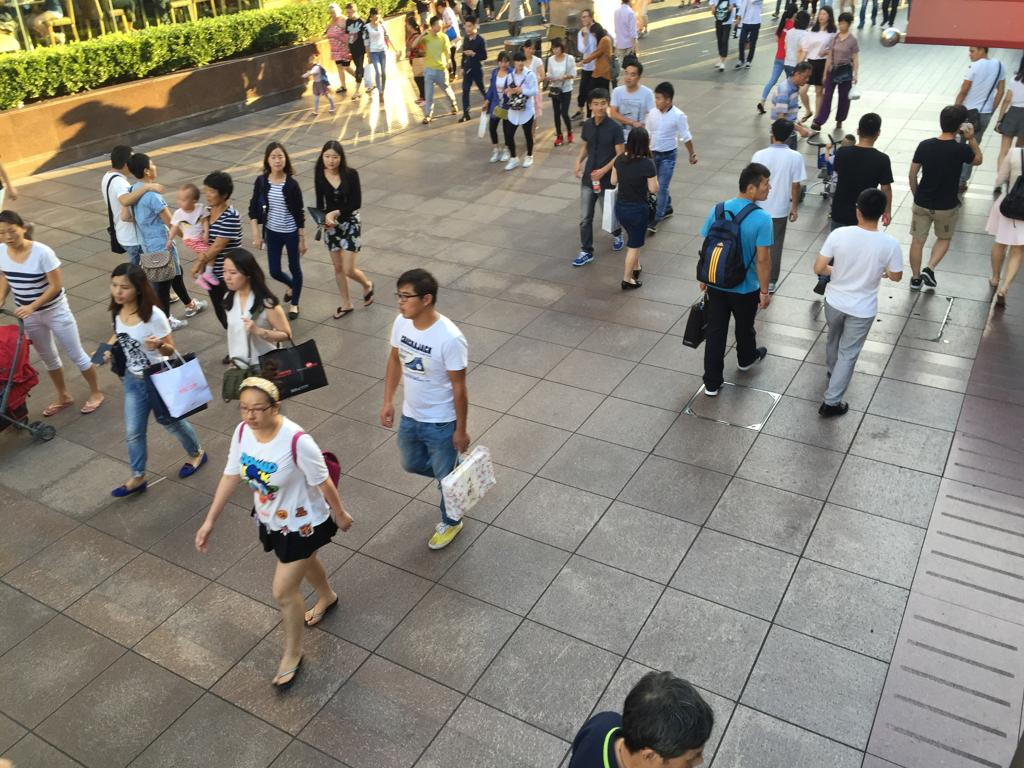
\includegraphics[width=\textwidth]{ornek2.jpg}
			\caption{Örnek 2}
			\label{Ornek2}
		\end{subfigure}
	\end{figure}
	
	
		\begin{figure}[!h]
			\subcaptionsetup{labelformat=empty}
				\begin{subfigure}{\textwidth}
			\raggedright
			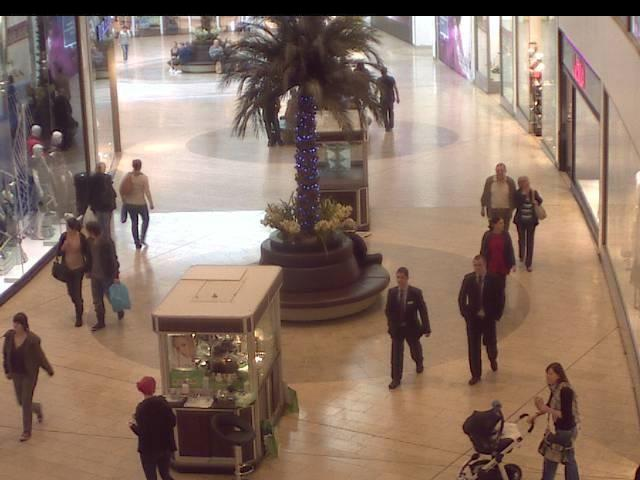
\includegraphics[width=\textwidth]{ornek3.jpg}
			\caption{Örnek 3}
			\label{Ornek3}
		\end{subfigure}
		\begin{subfigure}{\textwidth}
			\raggedright
			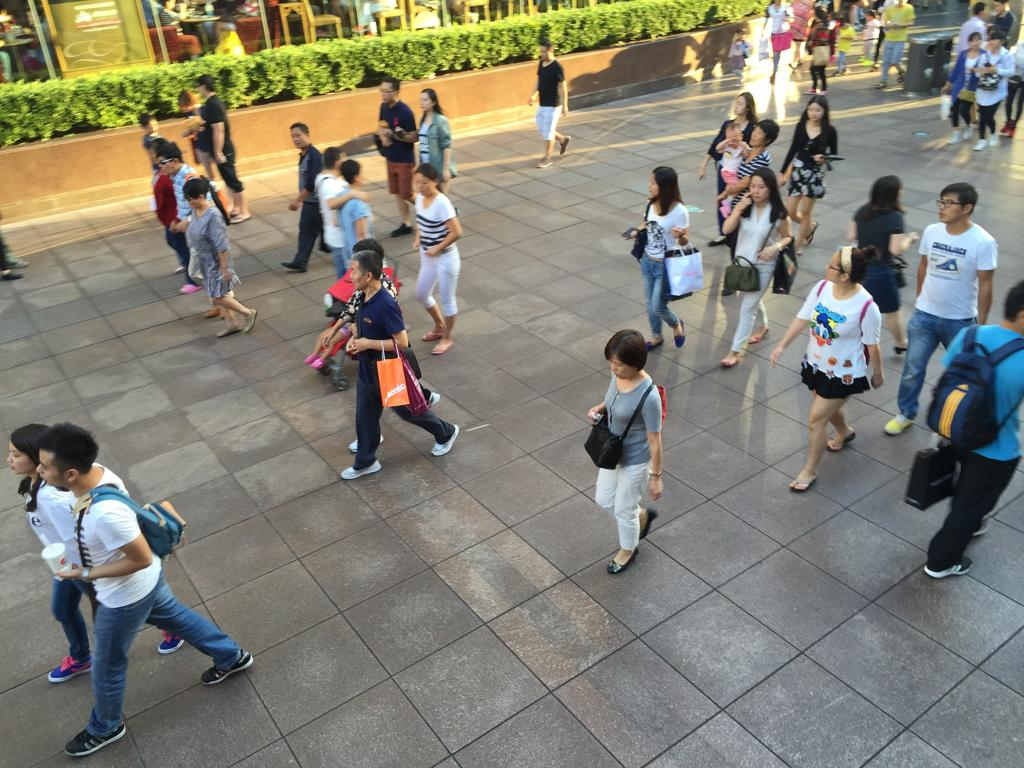
\includegraphics[width=\textwidth]{ornek4.jpg}
			\caption{Örnek 4}
			\label{Ornek4}
		\end{subfigure}
	\end{figure}


	\begin{figure}[!h]
		\subcaptionsetup{labelformat=empty}
		\begin{subfigure}{\textwidth}
			\raggedright
			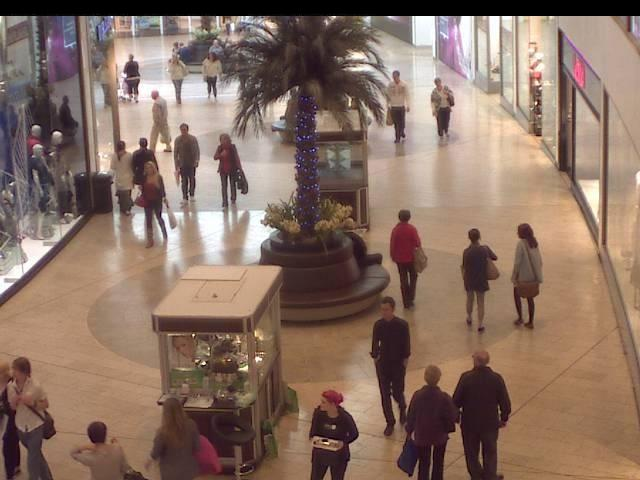
\includegraphics[width=\textwidth]{ornek5.jpg}
			\caption{Örnek 5}
			\label{Ornek5}
		\end{subfigure}
		\begin{subfigure}{\textwidth}
			\raggedright
			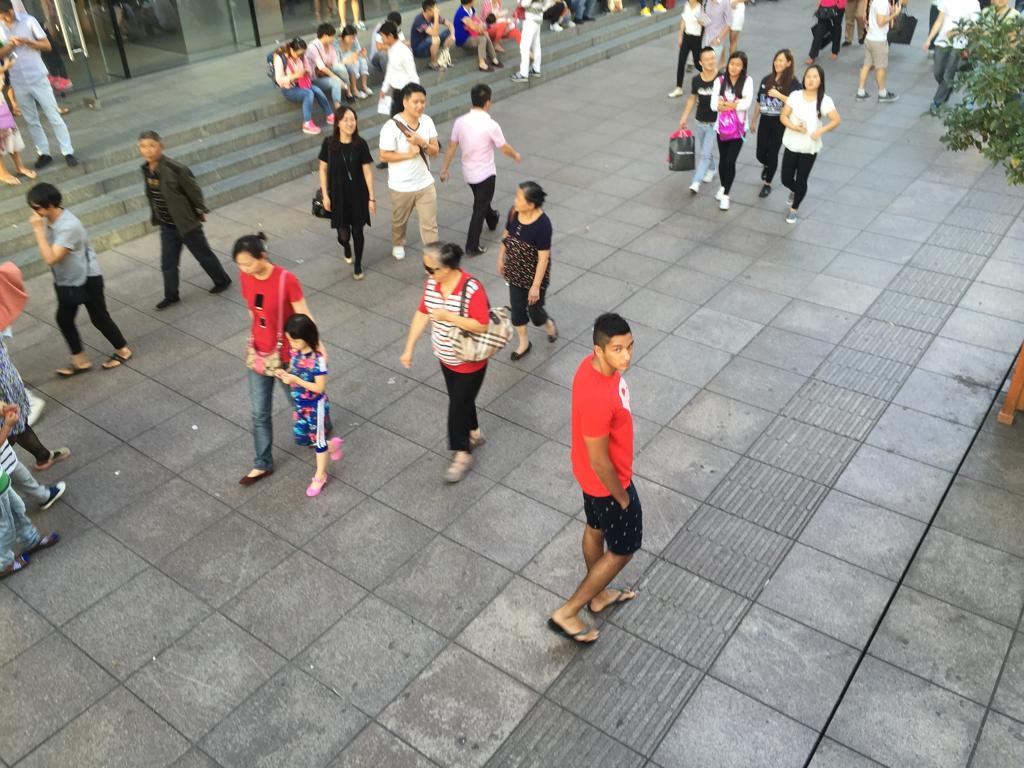
\includegraphics[width=\textwidth]{ornek6.jpg}
			\caption{Örnek 6}
			\label{Ornek6}
		\end{subfigure}
	\end{figure}
		
	 	\begin{figure}[!h]
			
			\raggedright
			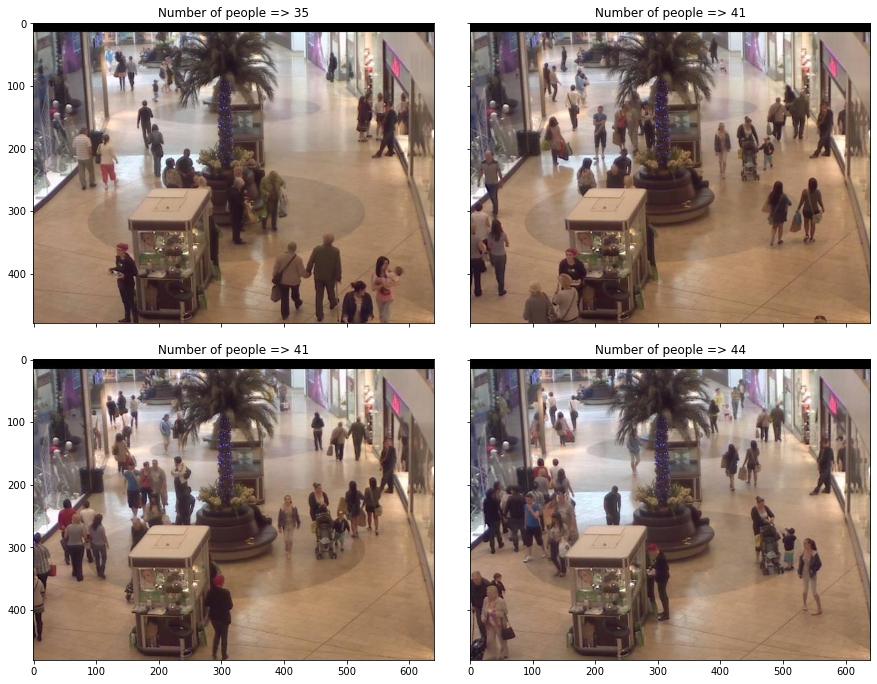
\includegraphics[width=\textwidth]{Ornek_sonuc1.png}
			\caption{Örnek}
			\label{Ornek_sonuc1}
		\end{figure}
		
		\begin{figure}[!h]
			
			\raggedright
			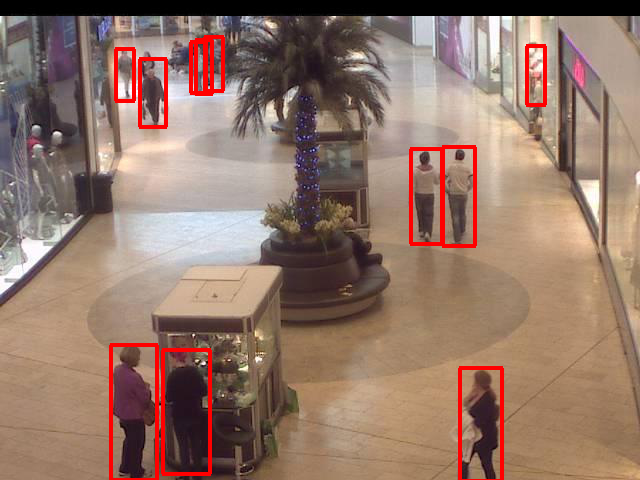
\includegraphics[width=\textwidth]{Ornek_sonuc2.png}
			\caption{Örnek}
			\label{Ornek_sonuc2}
		\end{figure}
		
		

		
		\begin{landscape}
					\begin{figure}[!h]
				
				\raggedright
				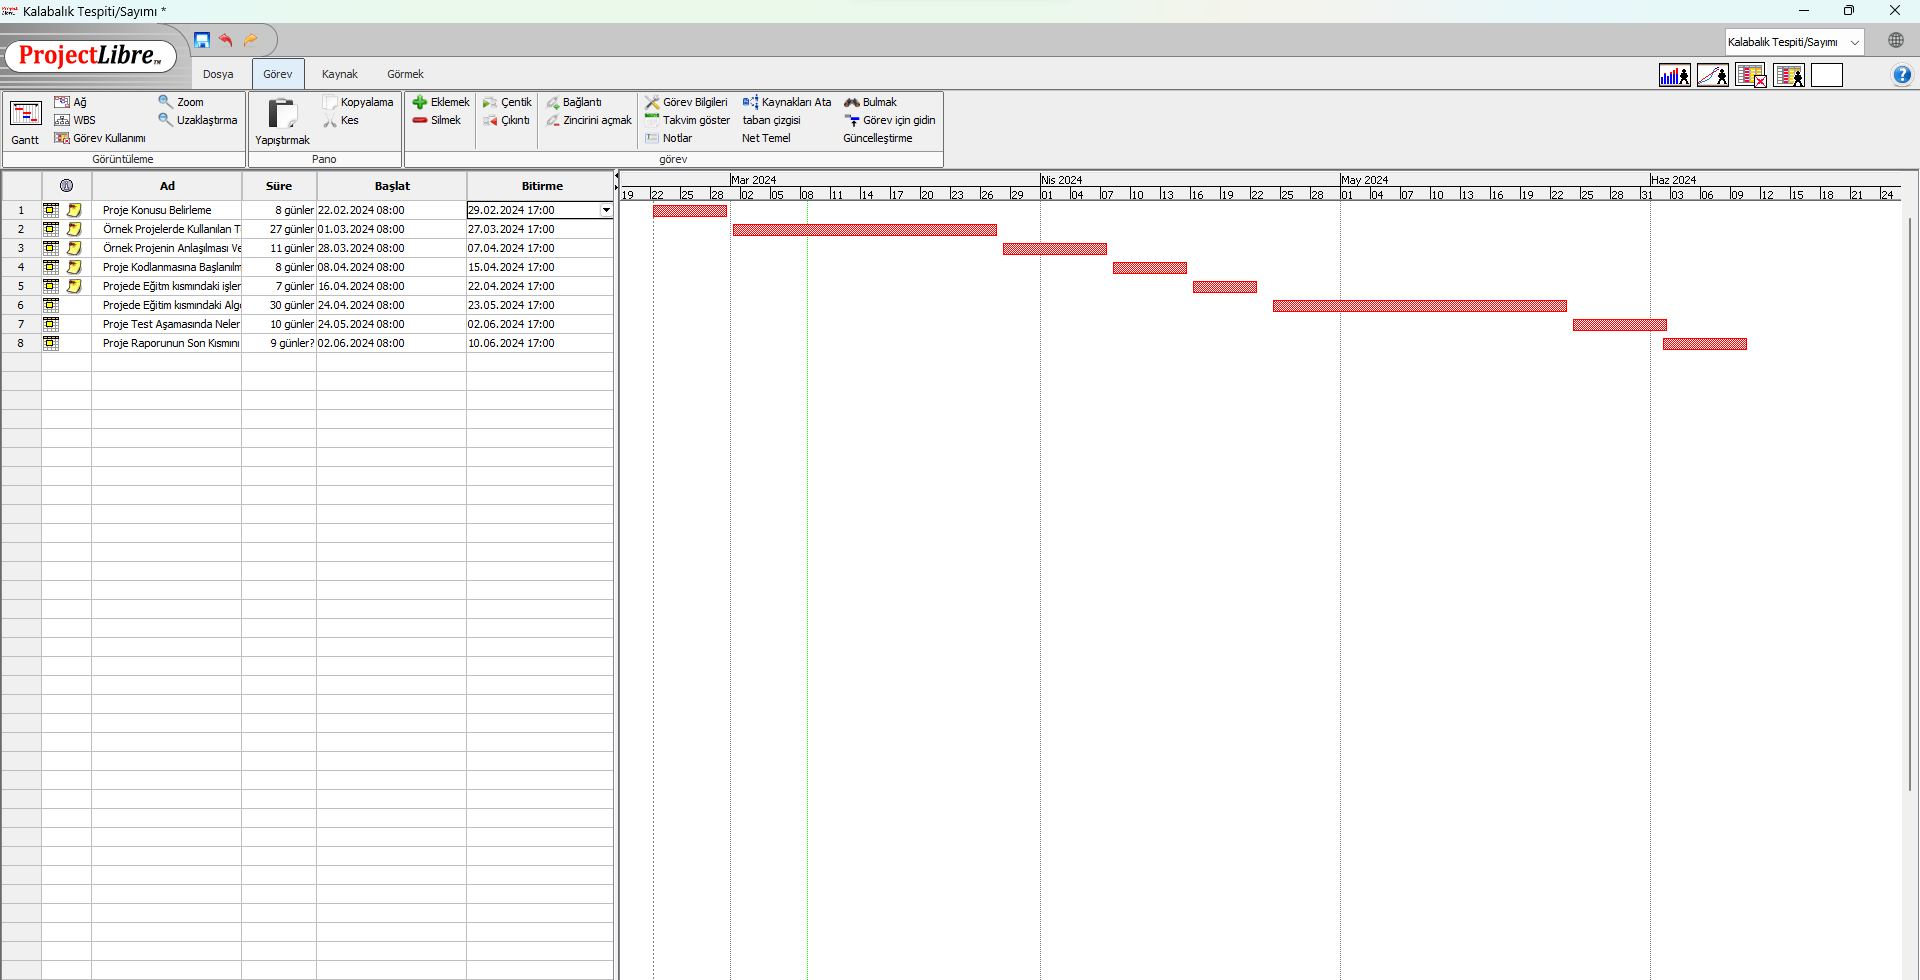
\includegraphics[height=\textheight]{GanttChart.png}
				\caption{İş Planı}
				\label{GanttChart}
			\end{figure}
		\end{landscape}
		
		\newpage
\begin{figure}[!h]
	\centering
	\begin{adjustbox}{width=\textwidth}
		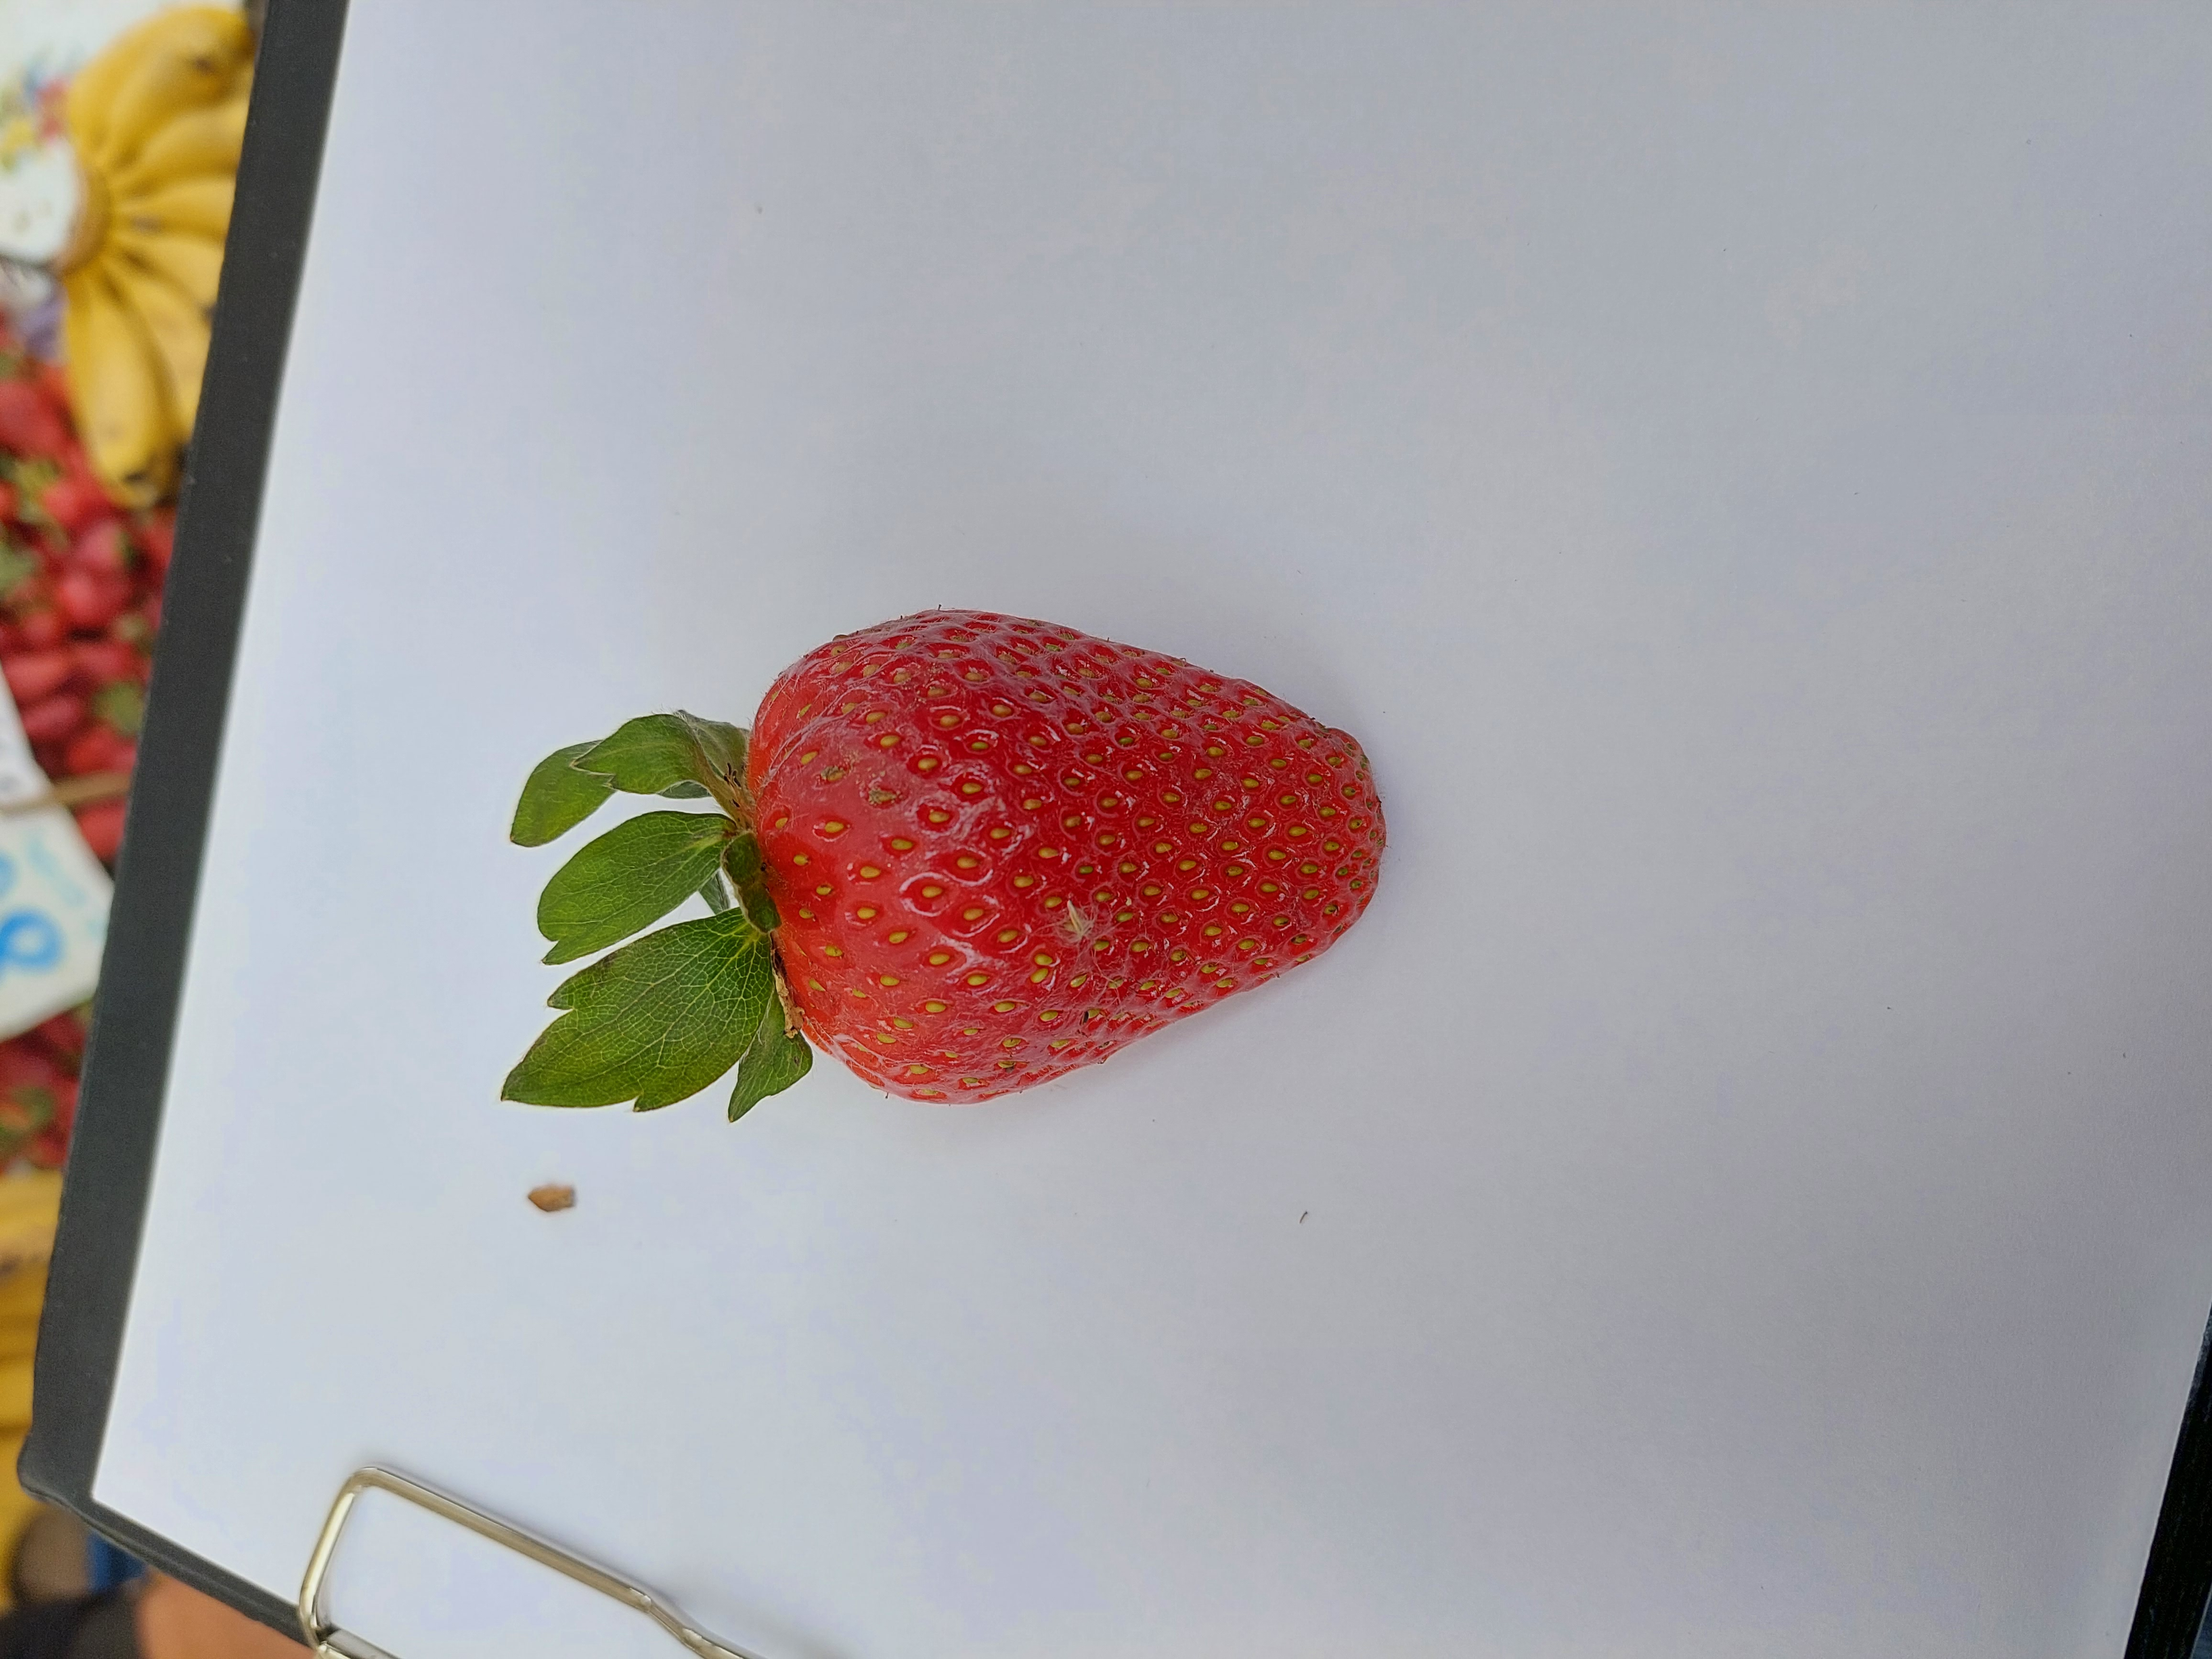
\includegraphics{resim1.png}
	\end{adjustbox}
	\caption{İş akış şeması}
	\label{resim1}
\end{figure}
	\newpage
		
		
\raggedright	\section*{4. Beklenen Sonuçlar}
			
			
	\begin{enumerate}
			\item[\textbf{4.1}] \textbf{Hassasiyet ve Doğruluk}	
			
				
					Modelin eğitim aşamasında ve sonrasında elde edilen sonuçlar, kalabalık sayımında  hassasiyet ve doğruluk seviyeleri Gerçek hayatta kabul edilebilir değerler olmalıdır Figure: \ref{Ornek_sonuc2}'deki gibi.\\
					
			\item[\textbf{4.2}] \textbf{Transfer Öğrenme Etkinliği}		
				
			  	   Önceden eğitilmiş ResNet50 veya diğer modellerin transfer öğrenme yönteminin etkinliği değerlendirilmelidir. Başka bir görevde eğitilen model kullanılıyorsa kalabalık sayma probleminde ne kadar başarılı olduğunu gösteren sonuçlar elde edilmelidir.
					
					
					
			\item[\textbf{4.3}] \textbf{Regresyon Performansı}	
					
					Regresyon kullanılarak elde edilen sonuçlar incelenmeli ve giriş görüntülerindeki insan sayısının sürekli, bir değer olarak doğru bir şekilde tahmin edilip edilmediği değerlendirilmelidir.		

			\item[\textbf{4.4}] \textbf{Kullanılan Teknolojiler-Kütüphaneler}
			
			
				   Keras, TensorFlow, scikit-learn, NumPy, Pandas, Seaborn, SciPy, Matplotlib gibi kullanılan teknoloji ve kütüphanelerin etkin bir şekilde kullanılması ve entegrasyonu gösterilmelidir.			
					
				
					
					
	\end{enumerate}




	\bibliographystyle{plain}
	\bibliography{references.bib} 
\end{document}